% !Mode::"TeX:UTF-8"
% !Mode:: "TeX:UTF-8"
\documentclass[xcolor=svgnames,serif,table,10pt]{beamer}
\mode<presentation>{
% Setup appearance:
\useoutertheme{infolines}
\usetheme{Darmstadt}
\setbeamercovered{transparent}
\setbeamertemplate{caption}[numbered]
\setbeamertemplate{navigation symbols}{}
\setbeamertemplate{blocks}[rounded][shadow=true]
\setbeamertemplate{enumerate items}[circle]

% 修改样式
\setbeamercolor{box}{bg=black!20!orange,fg=white}
\setbeamercolor{block title}{use=sidebar,fg=sidebar.fg!10!white,bg=orange!70!black}
\setbeamercolor{block title example}{use=sidebar,fg=sidebar.fg!10!white,bg=black!60!green}
\setbeamercolor{block title alerted}{use=sidebar,fg=sidebar.fg!10!white,bg=black!50!red}

\setbeamertemplate{headline}
{%
  \begin{beamercolorbox}[shadow=true]{section in head/foot}
  \vskip2pt\insertnavigation{\paperwidth}\vskip2pt
  \end{beamercolorbox}%
}
}
\usepackage{url}
\usepackage{animate}
\usepackage[english]{babel}
\usepackage{times}
\usepackage[T1]{fontenc}
\usepackage{multirow,multicol,longtable}
\usepackage{graphics}
\usepackage{xcolor}
\usepackage[no-math]{fontspec}%-------------------------------------------------- 提供字体选择命令
\usepackage{xunicode}%----------------------------------------------------------- 提供Unicode字符宏
\usepackage{xltxtra}%------------------------------------------------------------ 提供了针对XeTeX的改进并且加入了XeTeX的LOGO
\usepackage[BoldFont,SlantFont,CJKchecksingle]{xeCJK}%--------------------------- 使用xeCJK宏包


%================================== 设置中文字体 ================================%
%\setCJKmainfont{Adobe Heiti Std}%------------------------------------------------设置正文为黑体
%\setCJKmonofont{Adobe Song Std}%-------------------------------------------------设置等距字体
%\setCJKsansfont{Adobe Kaiti Std}%------------------------------------------------设置无衬线字体
% \setCJKfamilyfont{zxzt}{FZShouJinShu-S10S}
% \setCJKfamilyfont{FZDH}{FZDaHei-B02S}
%================================== 设置中文字体 ================================%

%================================== 设置英文字体 ================================%
\setmainfont[Mapping=tex-text]{Times New Roman}%--------------------------------英文衬线字体
\setsansfont[Mapping=tex-text]{Arial}%------------------------------------英文无衬线字体
\setmonofont[Mapping=tex-text]{Courier New}%-------------------------------------英文等宽字体
\newfontfamily\Arial{Arial}
%================================== 设置英文字体 ================================%

%================================== 设置数学字体 ================================%
%\setmathsfont(Digits,Latin,Greek)[Numbers={Lining,Proportional}]{Minion Pro}
%================================== 设置数学字体 ================================%
\punctstyle{kaiming}%------------------------------------------------------------ 开明式标点格式
\usepackage{graphicx}
\usepackage{tikz}
\usetikzlibrary{positioning,backgrounds}
\usetikzlibrary{fadings}
\usetikzlibrary{patterns}
\usetikzlibrary{calc}
\usetikzlibrary{shadings}
\pgfdeclarelayer{background}
\pgfdeclarelayer{foreground}
\pgfsetlayers{background,main,foreground}
\usepackage{xifthen}
\usepackage{colortbl,dcolumn}
\usepackage{enumerate}
\usepackage{pifont}
\usepackage{tabularx}
\usepackage{booktabs}
\usepackage{hyperref}
%=================================== 数学符号 =================================%
\newcommand{\rtn}{\mathrm{\mathbf{R}}}
\newcommand{\N}{\mathrm{\mathbf{N}}}
\newcommand{\As}{\mathrm{a.s.}}
\newcommand{\Ae}{\mathrm{a.e.}}
\newcommand*{\PR}{\mathrm{\mathbf{P}}}
\newcommand*{\EX}{\mathrm{\mathbf{E}}}
\newcommand{\EXlr}[1]{\mathrm{\mathbf{E}}\left[#1\right]}
\newcommand*{\dif}{\,\mathrm{d}}
\newcommand*{\F}{\mathcal{F}}
\newcommand*{\h}{\mathcal{H}}
\newcommand*{\vp}{\varepsilon}
\newcommand*{\prs}{\dif\PR-\As}
\newcommand*{\dte}{\dif t-\Ae}
\newcommand*{\pts}{\dif\PR\times\dif t-\Ae}
\newcommand{\Ito}{It\^{o}}
\newcommand{\tT}[1][0]{[#1,T]}
\newcommand{\intT}[2][T]{\int^{#1}_{#2}}
\newcommand{\intTe}[1][t]{\intT[t+\varepsilon]{#1}}
\newcommand{\s}{\mathcal{S}}
\newcommand{\me}{\mathrm{e}}
\newcommand{\one}[1]{{\bf 1}_{#1}}
\renewcommand{\M}{{\rm M}}
\newcommand{\Me}[1][t]{M^{\varepsilon}_{#1}}
\newcommand{\Ne}[1][t]{N^{\varepsilon}_{#1}}
\newcommand{\Pe}[1][t]{P^{\varepsilon}_{#1}}
\DeclareMathOperator*{\sgn}{sgn}
% =================================== 数学符号 =================================%

% 定义罗马数字
\makeatletter
\newcommand{\rmnum}[1]{\romannumeral #1}
\newcommand{\Rmnum}[1]{\expandafter\@slowromancap\romannumeral #1@}
\makeatother

% 定义破折号
\newcommand{\pozhehao}{\kern0.3ex\rule[0.8ex]{2em}{0.1ex}\kern0.3ex}
% 中文日期
\def\CJK@today{\the\year 年 \the\month 月}
\newcommand\zhtoday{\CJK@today}

% 中文图表
\renewcommand\figurename{图}
\renewcommand\tablename{表}

\graphicspath{{fig/},} 

% Author, Title, etc.

\title{信号检测与估值}

%% \subtitle{Foreground-constrained Eulerian Video Motion Magnification}

\author[段江涛]{段江涛
\\机电工程学院}

\institute[LSEC,AMSS,CAS]{
\includegraphics[height=1cm]{xd.jpg}}

\date{\zhtoday}

\setlength{\baselineskip}{22pt}
\renewcommand{\baselinestretch}{1.4}

% The main document

\begin{document}
\setlength{\abovedisplayskip}{1ex}%------------------------------------------ 公式前的距离
\setlength{\belowdisplayskip}{1ex}%------------------------------------------ 公式后的距离

\begin{frame}
  \titlepage
\end{frame}

%%%%%%%%%%%%%%%%%%%%%%%%%%%%%%%%5
%%%%%%%%%%%%%%%%%%%%%%%%%%% ch2
\begin{frame}[shrink]
\frametitle{ch2.信号检测与估计理论的基础知识}
\framesubtitle{概率论简单回顾}
\tableofcontents[hideallsubsections]
\end{frame}


\section{样本空间,事件域,概率}

\begin{frame}{随机现象}
随机现象:\\
~\\
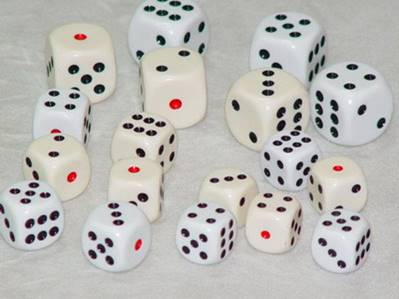
\includegraphics[scale=0.5]{die1}
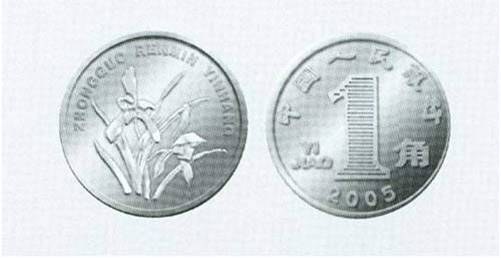
\includegraphics[scale=0.5]{coin1}\\
落叶的运动轨迹,气泡的扩散,灯泡的寿命
\begin{block}{随机现象特点}
	至少两种可能; 不确定性。
\end{block}
\end{frame}

\begin{frame}{概率论中的三个组成部分}
\begin{itemize}
	\item 样本空间$\Omega$
	\item 事件域$\mathcal{F}$
	\item 概率$P$
\end{itemize}
\end{frame}

\begin{frame}
\begin{itemize}
	\item 样本空间$\Omega$:一个随机试验所有可能出现的结果的全体,称为随机事件的样本空间。\\
	每一个可能的结果称为基本事件,它们的全体就是样本空间。
	\item 样本点$\xi_k$:随机试验的一个结果,就是某个基本事件,也就是$\Omega$中的一个元素。\\
	$\Omega=\{\xi_k|k=1,\dots,n\}$
	\item 随机事件$A$: 样本空间中的某个子集称为随机事件,简称事件(事件是集合)。
    \item 事件域$\mathcal{F}$: 样本空间中的某些子集构成的满足如下条件的集合,称为事件域(又称$\sigma^-$域)。
	\begin{itemize}
		\item[(1)] $\Omega\in\mathcal{F}$
		\item[(2)] 若$A\in\mathcal{F}$, 则$A$的补$\overline{A}\in\mathcal{F}$
		\item[(3)] 若$A_n\in\mathcal{F}, n=1,2,\dots$, 则$\bigcap\limits_{n=1}^{\infty}A_n\in\mathcal{F}$
	\end{itemize}
\end{itemize}
\end{frame}

\begin{frame}
\begin{example}
	一个盒子中有10个相同的球,5各白色,5个黑色,搅匀后从中任意摸取一球。\\
	$\xi_1=\{\text{取得白球} \}$, $\xi_2=\{\text{取得黑球} \}$\\
	$\Omega=\{\xi_1,\xi_2\}$
\end{example}
\begin{example}
	一个盒子中有10个相同的球,编号1,2,...,10, 从中取一球。\\
	$\Omega=\{1,2,\dots,10\}$\\
	$A=\{\text{6号球} \}=\{6\}$, $B=\{\text{偶数编号球} \}=\{2,4,6,8,10\}$, $\overline{B}=\{\text{奇数编号球}\}$,$C=\{\text{编号小于等于5的球} \}=\{1,2,3,4,5\}$\\
	事件A是基本事件,而B和C则由多个基本事件所组成,并且$A,B,C\subset\Omega$。
\end{example}
\textit{空集$\emptyset$可以看作$\Omega$的子集,在任意一次试验中不可能有此事件发生,称为不可能事件。}
\end{frame}

\begin{frame}{事件$A$的概率$P(A)$}
  事件域中的元素就是随机事件。如果这些事件的随机性能够由定义在$\mathcal{F}$上的具有非负性,归一性和可列加性的实函数$P(A)$来确定,则称$P$是定义在二元组$(\Omega,\mathcal{F})$上的概率,而称$P(A)$为事件$A$的概率。
  \begin{enumerate}
  	\item[(1)] 非负性。 $P(A)\ge 0$
  	\item[(2)] 归一性。 $P(\Omega)=1$
    \item[(3)] 可列加性。$A_1,A_2,...,A_n$互不相容$(A_i\cap A_j=\emptyset,i\ne j)$,则$P(A_1\cup A_2\cup\dots\cup A_n) = P(A_1)+P(A_2)+\cdots+P(A_n)$
  \end{enumerate}
\end{frame}

\begin{frame}
\frametitle{古典概型}
\begin{itemize}
	\item 样本空间的元素(即基本事件)只有有限个,不妨设为$n$个,$\Omega=\{\xi_1,\xi_2,\dots,\xi_n\}$
	\item 每个基本事件出现的可能性是相等的,即有$P(\xi_1)=P(\xi_2)=\cdots=P(\xi_n)$
	\item 事件域$\mathcal{F}$为$\Omega$的所有子集的全体,即是$Pwr(\Omega),\Omega$的幂集,共有$2^n$个事件,$\emptyset\in\mathcal{F},\Omega\in\mathcal{F}$。
	\item 由概率的有限可加性知\\
	$1=P(\Omega)=\sum\limits_{i=1}^{n}P(\xi_i)\implies P(\xi_i)=\frac{1}{n},(i=1,\dots,n)$
	\item 对任意一个随机事件$A\subseteq\mathcal{F}$, 如果$A$是$k$个基本事件的和,即$A=\{\xi_{i_1}\}\cup \{\xi_{i_2}\}\cup\cdots\cup\{\xi_{i_k}\}$, 则
	$$P(A)=\frac{k}{n}=\frac{\text{$A$中所包含的基本事件数}}{\text{基本事件总数}}$$
\end{itemize}
\end{frame}

\begin{frame}
\frametitle{样本空间的选取}
为求一个事件的概率,样本空间可以有不同的取法,但一定要认真,基本事件和求概事件数的计算都要在同一个样本空间中进行,否则会导致谬误!
\begin{example}
	一个盒子中有10个相同的球,编号1,2,...,10, 从中取一球,求此球的号码为偶数的概率。\\
	$\Omega=\{1,2,\dots,10\}$\\
	$A=\{\text{偶数编号球} \}=\{2\}\cup\{4\}\cup\{6\}\cup\{8\}\cup\{10\}=\{2,4,6,8,10\}$。\\
	$P(A)=\frac{|A|}{n}=\frac{5}{10}=\frac{1}{2}$
\end{example}
另外一种解法:$\Omega=\{A,\overline{A}\},A=\{\text{编号为偶数的球}\},\overline{A}=\{\text{编号为奇数的球}\},\mathcal{F}=\{\emptyset,\Omega,A,\overline{A}\}$,由$A,\overline{A}$的对称性,即得$P(A)=\frac{1}{2}$

\end{frame}

\begin{frame}
\frametitle{样本空间的选取}
\begin{block}{Notes}
	两种解法的样本空间$\Omega$不同(从而事件域$\mathcal{F}$是不同的)。严格地说,两者所描述的随机试验是不同的。例如对于第二种解法来说,$B=\{\text{号码为4的球}\}$并不属于事件域$\mathcal{F}$,就是说$B$不是一个事件,从而也就没有概率可言。但对第一种解法,$B$是事件,而且$P(B)=\frac{1}{10}$。
\end{block}
\end{frame}

\begin{frame}{几何概率}
我们在一个面积为$S_\Omega$的区域$\Omega$中,等可能地任意投点,如果点落入小区域$S_A$中的可能性与$S_A$成正比,而与$A$的位置及形状无关。如果``点落入小区域$A$"这个随机事件仍然记为$A$,则由$P(\Omega)=1$可得
$$P(A)=\frac{S_A}{S_\Omega}$$
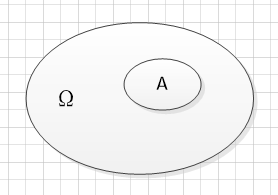
\includegraphics[scale=0.4]{geometry}
\end{frame}

\begin{frame}
\begin{example}
	(会面问题)甲、乙两人约定在6时到7时之间在某处会面,并约定先到者应等候另一个人一刻钟,过时即可离去。求两人能会面的概率。\\
	如图,以x,y表示甲乙两人,则两人能会面的充要条件是: $|x-y|\leq 15$\\
	$$P(A)=\frac{S_A}{S_\Omega}=\frac{60^2-45^2}{60^2}=\frac{7}{16}$$
	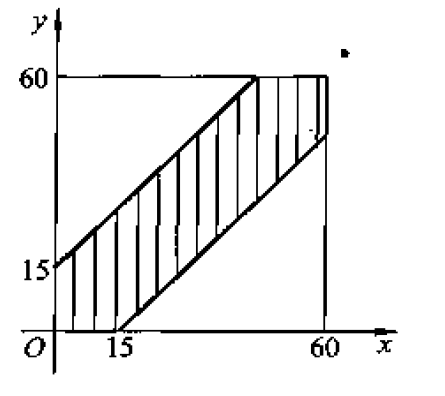
\includegraphics[scale=0.4]{geometry1}
\end{example}
\end{frame}

\section{几何概率与条件概率}

\begin{frame}{条件概率}
\begin{definition}
	若$\Omega,\mathcal{F},P$是一个概率空间,$B\in\mathcal{F}$, 且$P(B)>0$,则对任意的$A\in\mathcal{F}$,称
	$$P(A|B)=\frac{P(AB)}{P(B)}$$
	为在已知事件B发生的条件下,事件A发生的条件概率。
\end{definition}

\begin{columns}%0.6 0.4表示相对比例
	\column{0.4\textwidth}%<1->
\[P(A|B)=\frac{S_{AB}}{S_B}=\frac{S_{AB}/S_\omega}{S_B/S_\omega}=\frac{P(AB)}{P(B)} \]
	\column{0.4\textwidth}%<1->
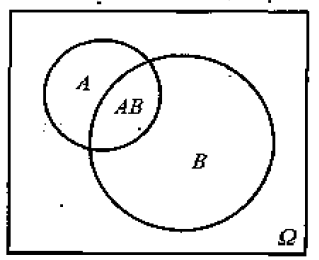
\includegraphics[scale=0.2]{P(AB)}
\end{columns}
\end{frame}

\begin{frame}{条件概率的性质及其推论}
\begin{block}{条件概率$P(\bullet|B)$的具备概率的三个基本性质}
	\begin{enumerate}
		\item 非负性: 对任意的$A\in F, P(A|B)\ge 0$;
		\item 规范性: $P(\Omega|B)=1$;
		\item 可列加性: 对任意的一列两两互不相容的事件$A_i(i=1,2,\dots)$, 有
		\[P\left[\bigcup\limits_{i=1}^{+\infty}(A_i|B)\right]=\sum\limits_{i=1}^{+\infty}P(A_i|B) \]
	\end{enumerate}
\end{block}
\begin{corollary}
概率的乘法公式:  $P(AB)=P(B)P(A|B)$
\end{corollary}

\begin{corollary}
	$P(A_1A_2\cdots A_n)=P(A_1)P(A_2|A_1)P(A_3|A_1A_2)\cdots P(A_n|A_1A_2\cdots A_{n-1})$
\end{corollary}
\end{frame}

\begin{frame}
\begin{example}
	一个家庭中有两个小孩,已知其中有一个是女孩,问这时另一个小孩也是女孩的概率有多大?\\
	$\Omega=$\{(男,男),(男,女),(女,男),(女,女)\}\\
	$A=$\{已知有一个是女孩\}=\{(男,女),(女,男),(女,女)\}\\
	$B=$\{另一个也是女孩\}=\{(女,女)\}\\
	于是所求概率为\\
	$P(B|A)=\frac{P(AB)}{P(A)}=\frac{1/4}{3/4}=\frac{1}{3}$
\end{example}
\end{frame}

\begin{frame}{概率树/全概率公式}
概率树思想:为了求解复杂事件的概率,往往可以先把它分解成两个(或若干个)互不相容的较简单的事件之并。求出这些较简单事件的概率,再利用加法公式即得所要求的复杂事件的概率。把这个方法一般化,便的到下述定理。
\begin{theorem}
	设$B_1,B_2,\cdots$是一列互不相容的事件,且有
	\[\bigcup_{i=1}^{+\infty}B_i=\Omega,P(B_i)>0 \]
	则对任一事件A,有
	\[P(A)=\sum_{i=1}^{+\infty}P(B_i)P(A|B_i) \]	
\end{theorem}
\end{frame}

\begin{frame}
\begin{example}
	某工厂有4条流水线生产同一种产品, 该4条流水线的产品分别占总产量的15\%, 20\%, 30\%, 35\%, 又这4条流水线的不合格品率依次为0.05, 0.04, 0.03及0.02. 现从出厂产品中任取一件, 问(1) 恰好抽到不合格品的概率为多少? (2) 第4条流水线应承担的责任?
\end{example}
\end{frame}

\begin{frame}[shrink]
解: (1) 令
\begin{align*}
A&=\{\text{任取一件,恰好抽到不合格品} \}\\
B&=\{\text{任取一件,恰好抽到第$i$条流水线的产品}, (i=1,2,3,4) \}
\end{align*}
于是由全概率公式可得
\begin{align*}
P(A)&=\sum\limits_{i=1}^4P(B_i)P(A|B_i)=0.15\times 0.05+0.20\times 0.04+0.30\times 0.03+0.35\times 0.02\\
&=0.0315=3.15\%
\end{align*}
实际上,$P(A|B_i)$可以从过去生产的产品中统计出来,称为先验概率。\\
(2) 从概率论的角度考虑可以按$P(B_i|A)$的大小来追究第$i$条$i=1,2,3,4$流水线的责任。\\
$P(AB_4)=P(B_4)P(A|B_4)=0.35\times 0.02=0.007$\\
由条件概率的定义知
\begin{align*}
P(B_4|A)=\frac{P(AB_4)}{P(A)}=\frac{P(B_4)P(A|B_4)}{\sum\limits_{i=1}^4P(B_i)P(A|B_i)}=\frac{0.007}{0.0315}\approx=0.222
\end{align*}
\end{frame}

\begin{frame}{贝叶斯(Bayes)公式}
\begin{theorem}
	若$B_1, B_2, \dots$为一系列互不相容的事件, 且
	\[\bigcup\limits_{i=1}^{+\infty}B_i=\Omega \]
	\[P(B_i)>0, i=1,2,\dots \]
	则对任一事件A, 有
	\[P(B_i|A)=\frac{P(B_i)P(A|B_i)}{P(A)}=\frac{P(B_i)P(A|B_i)}{\sum\limits_{j=1}^{+\infty}P(B_j)P(A|B_j)}, \quad i=1,2,\dots \]
\end{theorem}
$P(B_i)$是试验以前就已经知道的概率---\textbf{先验(先于试验)概率}。\\
条件概率$P(B_i|A)$反映了试验以后,对A发生的``来源''的各种可能性的大小---\textbf{后验概率}。
\end{frame}

\begin{frame}{相互独立事件}
条件概率: $P(B|A)=\frac{P(AB)}{P(A)}$\\
一般的概率乘法公式: $P(AB)=P(A)P(B|A)$\\
如果``事件B发生与否不受事件A的影响'': $P(B)=P(B|A)$\\
乘法公式变为: $P(AB)=P(A)P(B)$
\begin{definition}
对任意的两个事件A,B,若
\[P(AB)=P(A)P(B)\]
成立,则称事件A,B是相互独立的,简称为独立的。	
\end{definition}
\begin{block}{依这个定义,不难验证:}
	若A与B相互独立,则$\{\emptyset,A,\overline{A},\Omega\}$中的任意一个与$\{\emptyset,B,\overline{B},\Omega\}$中的任意一个仍相互独立。
\end{block}
\end{frame}

\begin{frame}[shrink]
		分别掷两枚均匀的硬币,令
		\begin{align*}
		A=\{\text{硬币甲出现正面} \}\quad	B=\{\text{硬币乙出现正面} \}
		\end{align*}
		验证事件$A,B$是相互独立的。
 \begin{proof}
			$$\text{样本空间}=\{\text{(正,正),(正,反),(反,正),(反,反)}\} $$
			共还有4个基本事件,它们是等可能的,各有概率为1/4,而\\
			\begin{align*}
			A&=\{\text{(正,正),(正, 反)}\} \\
			B&=\{\text{(正,正),(反, 正)}\} \\
			AB&=\{\text{正,正}\}
			\end{align*}
			由此知 \[P(A)=P(B)=\frac{1}{2}\]
			这时有 \[P(AB)=\frac{1}{4}=P(A)P(B)\]
			成立,所以A, B事件是相互独立的。
 \end{proof}
\end{frame}

\section{随机变量}

\begin{frame}
\begin{definition}
	设$(\Omega,\mathcal{F},P)$是一概率空间,$x(\xi)|\xi\in\Omega$是定义在$\Omega$上的单值实函数,如果对任一实数$x$, 集合$\{x(\xi)\le x\}\in\mathcal{F}$, 则称$x(\xi)$为$(\Omega,\mathcal{F},P)$上的一个\textbf{随机变量}。
	
	随机变量$x(\xi)$的定义域为样本空间$\Omega$,它的值域是实数R。所有随机变量$x(\xi)$实际上是一个映射,这个映射为每个来自概率空间的结果(样本点)$\xi$赋予一个实数$x$。这种映射必须满足条件:
	\begin{itemize}
		\item[(1)] 对任一$x$,集合$\{x(\xi)\le x\}$是这个概率空间中的一个事件,并有确定的概率$P\{x(\xi)\le x\}$;
		\item[(2)] $P\{x(\xi)=\infty \}=0$, $P\{x(\xi)=-\infty \}=0$
	\end{itemize}
	\begin{block}{Notes}
		随机变量$x(\xi)$就是试验结果(即样本点)和实数之间的一一对应关系。虽然在试验之前不能肯定随机变量$x(\xi)$会取哪一个数值,但是对于任一实数$a$, 我们可以研究$\{x(\xi)=a \}$发生的概率, 也就是$x(\xi)$取值的统计规律。
	\end{block}
\end{definition}
\end{frame}

\begin{frame}{随机变量的分布函数}
\begin{definition}
	设$x(\xi)$是随机变量, 对$\forall x\in\mathbb{R}$, 称函数
	\[F(x)=P\{x(\xi)\le x\}\]
	为随机变量$x(\xi)$的一维(累积)分布函数[(cumulative) distribution function]。
\end{definition}
\begin{block}{分布函数性质}
\begin{enumerate}
	\item 单调不减性: 对$\forall x_1<x_2$, 恒有$F(x_1)\le F(x_2)$
	\item 规范性: $F(-\infty)=\lim\limits_{x\to -\infty}F(x)=0$, $F(+\infty)=\lim\limits_{x\to +\infty}F(x)=1$
	\item 右连续性: 对$\forall x_0$, 恒有$F(x_0+0)=\lim\limits_{x\to x_0^+}F(x)=F(x_0)$
\end{enumerate}
\end{block}
\end{frame}

\begin{frame}{随机变量的概率密度函数}
\begin{definition}
	设连续随机变量$x(\xi)$的一维累积分布函数为$F(x)$, 如果$F(x)$对$x$的一阶导数存在,则有
	\[p(x)\mathop{=}^{def}\frac{dF(x)}{dx}\]
	式中, $p(x)$称为随机变量$x(\xi)$的一维概率密度函数, 简称概率密度函数(probability density function,p.d.f)
\end{definition}
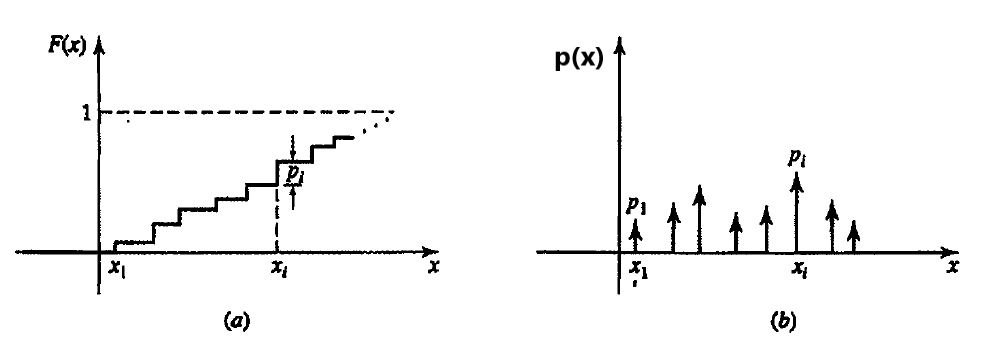
\includegraphics[scale=0.4]{pi}
\end{frame}

\begin{frame}[shrink]
\frametitle{随机变量概率密度函数性质}
\begin{enumerate}
	\item 根据随机变量$x(\xi)$的$p(x)$与$F(x)$的关系, 有
	\[F(x)=\int_{-\infty}^{x}p(u)du\]
	\item 对所有$x$, p(x)是非负函数,即
	\[p(x)\ge 0,\quad -\infty<x<+\infty \]
	\item $p(x)$对$x$的全域积分结果等于1, 一般表示为
	\[\int_{-\infty}^{\infty}p(x)dx=1\]
	\item 随机变量$x(\xi)$落在区间$[x_1,x_2]$内的概率为
	\[P\{x_1\le x(\xi)\le x_2\}=F(x_2)-F(x_1)=\int_{x_1}^{x_2}p(x)dx\]
\end{enumerate}
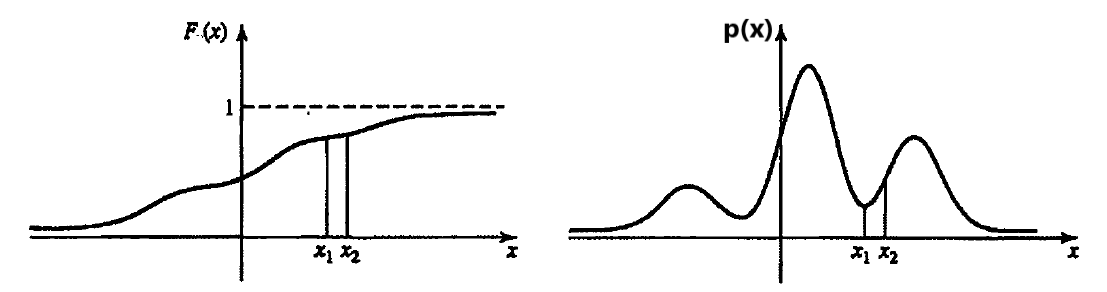
\includegraphics[scale=0.3]{Fx-px2}
\end{frame}

\begin{frame}[shrink]
抛掷一枚硬币: 样本空间: $\Omega=\{h,t\}$, $h$表示正面, $t$表示反面。正面的概率$p$, 反面的概率$q$. 定义随机变量$x(\xi),\xi\in \Omega$满足:
	\[x(\xi=h)=x(h)=1\qquad x(\xi=t)=x(t)=0,\]
	求$F(x)$,其中: $-\infty<x<\infty$.\\
	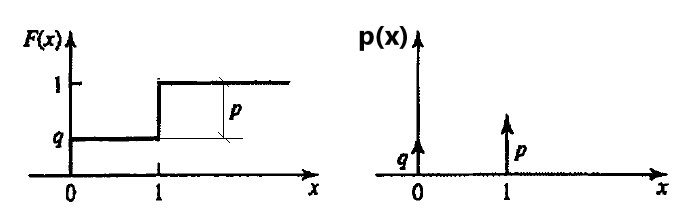
\includegraphics[scale=0.4]{coin-tossing}\\
	如果$x\ge 1$, 则$x(h)=1\le x$, 且$x(t)=0\le x$, 有
	\[F(x)=P\{x(\xi)\le x \}=P\{h,t\}=1\qquad x\ge 1 \] 
    如果$0\le x<1$, 则$x(h)=1> x$, 且$x(t)=0\le x$, 有
    \[F(x)=P\{x(\xi)\le x \}=P\{t\}=q \qquad 0\le x<1 \] 
    如果$x<0$, 则$x(h)=1> x$, 且$x(t)=0> x$, 有
    \[F(x)=P\{x(\xi)\le x \}=P\{\emptyset\}=0 \qquad x<0 \] 
\end{frame}

\begin{frame}[shrink]
事件A, 试验的样本空间: $\Omega=\{A,\overline{A},\emptyset \}$. 定义随机变量$x(\xi)$,
满足:
\begin{align*}
	x(\xi)=1, &\quad \xi\in A\\
	x(\xi)=0, &\quad \xi\in\overline{A}
\end{align*}
$P(A)=p,P(\overline{A})=q=1-p$
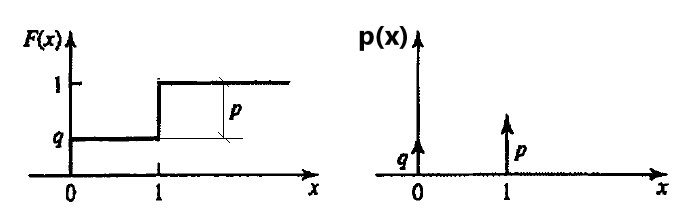
\includegraphics[scale=0.4]{coin-tossing}\\
如果$x\ge 1$, 则$\{x(\xi)\le x\}=\{\Omega \}$, 有
\[F(x)=P\{x(\xi)\le x \}=P\{\Omega \}=1\qquad x\ge 1 \] 
如果$0\le x<1$, 则$\{x(\xi)\le x\}=\{\overline{A}\}$, 有
\[F(x)=P\{x(\xi)\le x \}=P\{\overline{A}\}=q \qquad 0\le x<1 \] 
如果$x<0$, 则$\{x(\xi)\le x\}=\{\emptyset\}$, 有
\[F(x)=P\{x(\xi)\le x \}=P\{\emptyset\}=0 \qquad x<0 \] 
\end{frame}

\begin{frame}[shrink]
抛掷两枚硬币: 随机变量$x(\xi)$表示正面数目。求$F(x)$.\\
样本空间: $\Omega=\{HH,HT,TH,TT\}$, $H$表示正面, $T$表示反面。\\
随机变量$x(\xi)$: $x(HH)=2,\quad x(HT)=1, \quad x(TH)=1, \quad x(TT)=0$
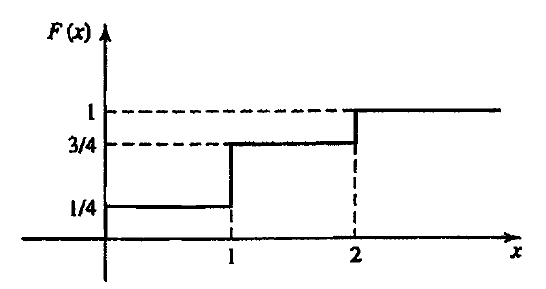
\includegraphics[scale=0.3]{coin-tossing2}\\
如果$x\ge 2$, $\{x(\xi)\le x\}=\Omega \Rightarrow F(x)=1$ \\
如果$1\le x<2$, $\{x(\xi)\le x\}=\{TT,HT,TH\} \Rightarrow F(x)=P\{TT\}+P\{HT\}+P\{TH\}=\frac{3}{4}$ \\
如果$0\le x<1$, $\{x(\xi)\le x\}=\{TT\} \Rightarrow F(x)=P\{TT\}=P(T)P(T)=\frac{3}{4}$ \\
如果$x<0$, $\{x(\xi)\le x \}=\emptyset \Rightarrow F(x)=0$ \\
当$x=1$, $P\{x(\xi)=1\}=F(1)-F(1^{-})=3/4-1/4=1/2$
\end{frame}

\begin{frame}[shrink]
掷一枚骰子: 样本空间: $\Omega=\{f_1,f_2,f_3,f_4,f_5,f_6\}$。定义随机变量$x(\xi),\xi\in \Omega$满足:$x(f_i)=10i$
求$F(x)$,其中: $-\infty<x<\infty$.\\
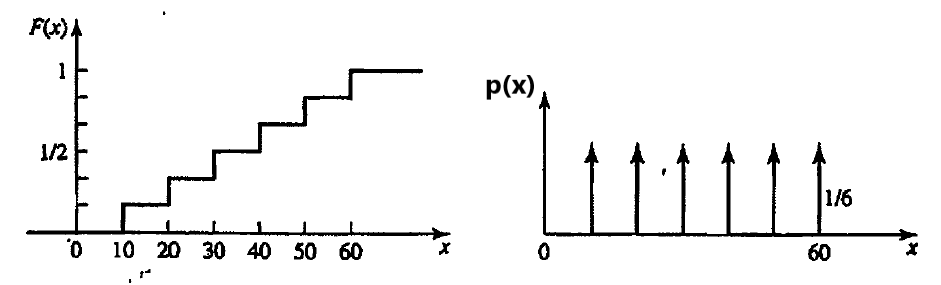
\includegraphics[scale=0.4]{die}
\begin{align*}
F(100)&=P\{x(\xi)\le 100 \}=P(\Omega)=1\\
F(35)&=P\{x(\xi)\le 35 \}=P\{f_1,f_2,f_3 \}=\frac{3}{6} \\
F(30.01)&=P\{x(\xi)\le 30.01 \}=P\{f_1,f_2,f_3 \}=\frac{3}{6} \\
F(30)&=P\{x(\xi)\le 30 \}=P\{f_1,f_2,f_3 \}=\frac{3}{6} \\
F(29.9)&=P\{x(\xi)\le 35 \}=P\{f_1,f_2 \}=\frac{2}{6} \\
\end{align*}
\end{frame}

\begin{frame}
\begin{columns}
	\column{0.5\textwidth}
	均匀分布随机变量$x(t)=t,0<t<T$\\
	$P\{t_1\le t\le t_2\}=\frac{t_2-t_1}{T},0<t_1<t_2<T$\\
	如果$x> T$, 有
	\[F(x)=P\{x(t)\le x \}=P\{0\le t\le T \}=P(\Omega)= 1\qquad x> 1 \] 
	如果$0\le x\le T$, 有
	\[F(x)=P\{x(t)\le x \}=P\{0\ge t\le x\}=\frac{x}{T} \qquad 0\le x\le 1 \] 
	如果$x<0$, 有
	\[F(x)=P\{x(t)\le x \}=P\{\emptyset\}=0 \qquad x<0 \] 
	\column{0.4\textwidth}
	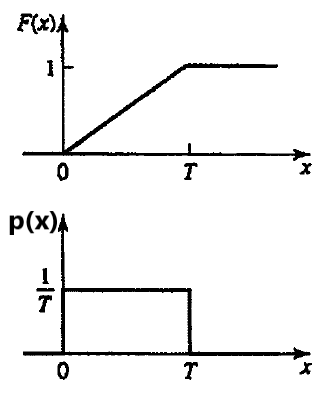
\includegraphics[scale=0.4]{xt}
\end{columns}
\end{frame}

\begin{frame}
\begin{columns}
	\column{0.5\textwidth}
	定义随机变量$x(\xi)$, 满足$\forall xi\in\Omega, x(\xi)=a$\\
	如果$x\ge a$, 则,$\forall \xi\in\Omega, x{\xi}=a\le x$,有
	\[F(x)=P\{x(\xi)\le x \}=P(\Omega)= 1\qquad x\ge a \] 
	如果$x<a$, 有
	\[F(x)=P\{x(t)\le x \}=P\{\emptyset\}=0 \qquad x<a \] 
	\column{0.4\textwidth}
	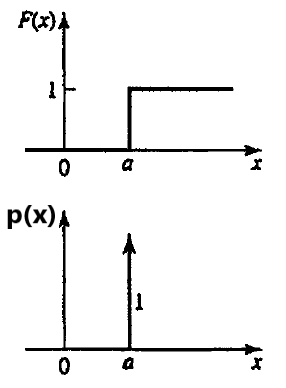
\includegraphics[scale=0.4]{a}
\end{columns}
\end{frame}

\begin{frame}[shrink]
非负实数集合$\{p_i\}$,$\forall i, i=1,2,\dots,\infty$满足, 
\begin{enumerate}
	\item $P\{x(\xi)=x_i\}=p_i$
	\item $\sum\limits_{i=1}^{\infty}p_i=1$
\end{enumerate}
求$F(x)$,其中: $-\infty<x<\infty$.\\
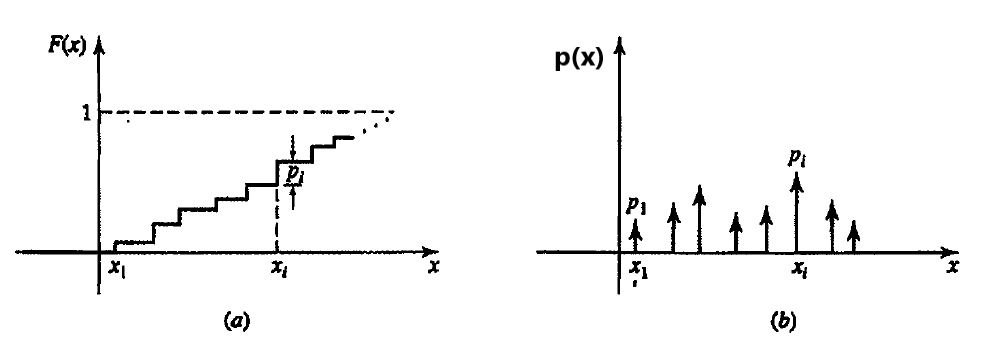
\includegraphics[scale=0.4]{pi}\\
对于$x_i\le x<x_{i+1}$, 我们有$\{x(\xi)\le x \}=\bigcup\limits_{x_k\le x}\{x(\xi)=x_k\}=\bigcup\limits_{k=1}^{i}\{x(\xi)=x_k\}$, 因此
\begin{align*}
F(x)=P\{x(\xi)\le x\}=\sum\limits_{k=1}^{i}p_k \qquad x_i\le x<x_{i+1}
\end{align*}
\end{frame}

\begin{frame}{离散型随机变量$x(\xi)$的$p(x)$}
\[P\{x(\xi)=x_i\}=F(x_j)-F(x_i^{-})=p_i\]
\[p(x)=\sum\limits_{i}p_i\delta(x-x_i) \]
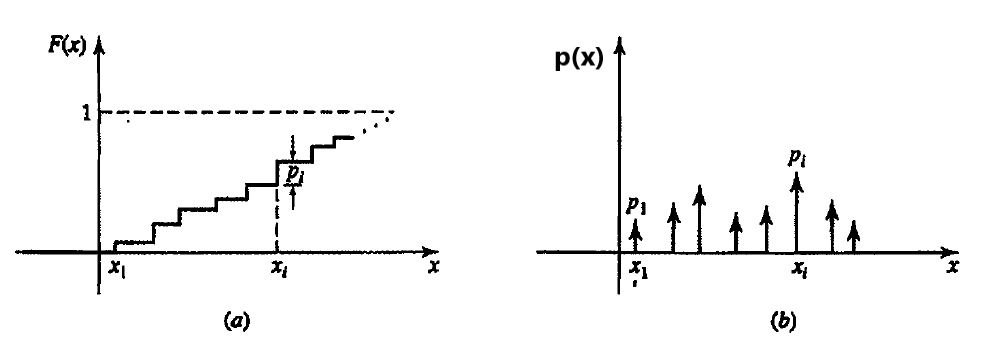
\includegraphics[scale=0.3]{pi}\\
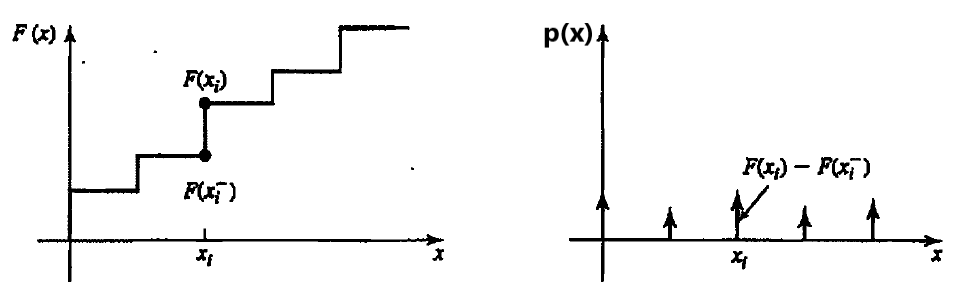
\includegraphics[scale=0.3]{Fx-px}
\end{frame}



%%%%%%%%%%%%%%%%%%%%%%%%%% ch3
\begin{frame}
  \frametitle{主要内容}
  \tableofcontents[hideallsubsections]
\end{frame}

\section{准备知识}
\begin{frame}
\begin{theorem}
	如果函数$f(x)$在区间$[a,b]$上连续,则积分上限函数
	\[\Phi(x)=\int_a^x f(t)dt\]
	在[a,b]上具有导数,并且它的导数是
	\[\Phi^\prime(x)=\frac{d}{dx}\int_a^xf(t)dt=f(x)\qquad (a\le x\le b) \]
\end{theorem}
\begin{theorem}
	如果函数$f(x)$在区间$[a,b]$上连续,则函数
	\[\Phi(x)=\int_a^x f(t)dt\]	
	就是$f(x)$在$[a,b]$上的一个原函数。
\end{theorem}
\end{frame}

\begin{frame}
\begin{theorem}
	如果函数$F(x)$是连续函数$f(x)$在区间$[a,b]$上的一个原函数,则
	\[\int_a^b f(x)dx=F(b)-F(a)\]	
\end{theorem}
\end{frame}

\begin{frame}
似然比检验的判别式:
\[\lambda(x)=\frac{p(x|H_1)}{p(x|H_0)}\mathop{\gtrless}_{H_0}^{H_1}\eta \]
判决概率:
\[P_F=P(H_1|H_0)=\int_{\eta}^{\infty}p(\lambda|H_0)d\lambda \]
\[P_D=P(H_1|H_1)=\int_{\eta}^{\infty}p(\lambda|H_1)d\lambda \]
\end{frame}

\begin{frame}
\begin{align*}
&P_D =P_D=P(H_1|H_1)=\int_{\eta}^{\infty}p(\lambda|H_1)d\lambda=P_D(\eta) \\
&P_F =P(H_1|H_0)=\int_{\eta}^{\infty}p(\lambda|H_0)d\lambda=P_F(\eta) \\
&\frac{dP_D(\eta)}{d\eta} =-p(\eta|H_1) \\ 
&\frac{dP_F(\eta)}{d\eta} =-p(\eta|H_0) \\ 
&\qquad \text{ by } \Phi^\prime(x)=\frac{d}{dx}\int_a^xf(t)dt=f(x)\qquad (a\le x\le b) \\
&\frac{dP_D(\eta)}{dP_F(\eta)} =\frac{-p(\eta|H_1)}{-p(\eta|H_0)}=\frac{p(\eta|H_1)}{p(\eta|H_0)}\\
\end{align*}
\end{frame}

\begin{frame}
\begin{align*}
P_D(\eta) &=P[(\lambda|H_1)\ge\eta]&\\
&=\int_{\eta}^{\infty}p(\lambda|H_1)d\lambda&\\
&=\int_{R_1}^{\infty}p(x|H_1)dx&\\
&=\int_{R_1}^{\infty}\lambda p(x|H_0)dx &\text{ by }\lambda(x)=\frac{p(x|H_1)}{p(x|H_0)}\mathop{\gtrless}_{H_0}^{H_1}\eta&\\
&=\int_{\eta}^{\infty}\lambda p(\lambda|H_0)d\lambda&
\end{align*}
\[\frac{dP_D(\eta)}{d\eta}=-\eta p(\eta|H_0)\]
\[\frac{dP_D(\eta)}{dP_F(\eta)}=\frac{-p(\eta|H_1)}{-p(\eta|H_0)}=\frac{-\eta p(\eta|H_0)}{-p(\eta|H_0)}=\eta \]  
\end{frame}

\begin{frame}
$H_1$含随机变量$m$的似然比检验的判别式:
\[\lambda(x)=\frac{p(x|m; H_1)}{p(x|H_0)}=\frac{\int_{-\infty}^{\infty}p(x|m,H_1)p(m)dm}{p(x|H_0)}\mathop{\gtrless}_{H_0}^{H_1}\eta \]
\end{frame}

\begin{frame}
$p(m)$未知
\begin{align*}
&p(x|H_0)=(\frac{1}{2\pi\sigma_n^2})^{1/2}\exp(-\frac{x^2}{2\sigma_n^2})\\
&p(x|m;H_1)=(\frac{1}{2\pi\sigma_n^2})^{1/2}\exp(-\frac{(x-m)^2}{2\sigma_n^2})\\
&\lambda(x)=\frac{p(x|m; H_1)}{p(x|H_0)}\mathop{\gtrless}_{H_0}^{H_1}\eta\\
&\exp(\frac{2mx}{2\sigma_n^2}-\frac{m^2}{2\sigma_n^2})\mathop{\gtrless}_{H_0}^{H_1}\eta\\
&mx\mathop{\gtrless}_{H_0}^{H_1}\sigma_n^2\ln\eta+\frac{m^2}{2}
\end{align*}
\end{frame}

\begin{frame}
\begin{align*}
&m_0\le m\le m_1,m_0>0\\
&mx\mathop{\gtrless}_{H_0}^{H_1}\sigma_n^2\ln\eta+\frac{m^2}{2}\\
&l(x)=x\mathop{\gtrless}_{H_0}^{H_1}\frac{\sigma_n^2}{m}\ln\eta+\frac{m}{2}\mathop{=}^{def}\gamma^+\\
&\int_{\gamma^+}^{\infty}(\frac{1}{2\pi\sigma_n^2})^{1/2}\exp(-\frac{l^2}{2\sigma_n^2})dl=\alpha
\end{align*}
\end{frame}

\begin{frame}
\begin{align*}
&m_0\le m\le m_1,m_1<00\\
&mx\mathop{\gtrless}_{H_0}^{H_1}\sigma_n^2\ln\eta+\frac{m^2}{2}\\
&l(x)=x\mathop{\lessgtr}_{H_0}^{H_1}-\frac{\sigma_n^2}{|m|}\ln\eta-\frac{|m|}{2}\mathop{=}^{def}\gamma^-\\
&\int_{-\infty}^{\gamma^-}(\frac{1}{2\pi\sigma_n^2})^{1/2}\exp(-\frac{l^2}{2\sigma_n^2})dl=\alpha
\end{align*}
\end{frame}

\begin{frame}
若$m_0>0$, $m$仅取正值, 则在$P(H_1|H_0)=\alpha$的约束下, $P^{(m)}(H_1|H_1)$是最大的,其一致最大功效检验成立;\\
若$m_1<0$, $m$仅取负值, 则在$P(H_1|H_0)=\alpha$的约束下, $P^{(m)}(H_1|H_1)$也是最大的。
\end{frame}

\begin{frame}
若$m_0<0,m_1>0$, 即$m$取值可能为正或可能为负的情况下, 无论参量信号的统计检测,按$m$仅取正值设计,还是按$m$仅取负值设计,都有可能在某些$m$值下,   $P^{(m)}(H_1|H_1)$不满足最大的要求。\\
例如,按$m$取正设计信号检测系统,当$m$为正时,$P^{(m)}(H_1|H_1)$最大, 但当$m$为负时, $P^{(m)}(H_1|H_1)$可能最小。\\
因此, 这种情况下不能采用奈曼-皮尔逊准则来实际最佳检测系统。
\end{frame}

\begin{frame}
若$m_0<0,m_1>0$, 即$m$取值可能为正或可能为负,奈曼-皮尔逊准则不能保证$P^{(m)}(H_1|H_1)$最大要求。考虑把约束条件$P(H_1|H_0)=\alpha$分成两个$\alpha/2$, 假设$H_1成立$的判决域由两部分组成。判决表示式为
	\[|x|\mathop{\gtrless}_{H_0}^{H_1}\gamma \]

\begin{block}{}
	虽然双边检验比均值$m$假定为正确时的单边检验性能差,但是比均值$m$假定为错误时的单边检验性能要好的多。因此不失为一种好的折中方法。
\end{block}
\end{frame}

\begin{frame}{广义似然比检验}
\begin{align*}
&\text{似然函数}\\
&p(x|m;H_1)=(\frac{1}{2\pi\sigma_n^2})^{1/2}\exp(-\frac{(x-m)^2}{2\sigma_n^2})\\
&\text{对$m$求偏导,令结果等于零,即} \\
&\frac{\partial\ln p(x|m;H_1)}{\partial m}|_{m=\widehat{m}_{ml}}=0\\
&\text{解得单次观测时,$m$的最大似然估计量$\widehat{m}_{ml}=x$, 于是有 }\\
&p(x|\widehat{m}_{ml};H_1)=(\frac{1}{2\pi\sigma_n^2})^{1/2}\exp(-\frac{(x-\widehat{m}_{ml})^2}{2\sigma_n^2})|_{\widehat{m}_{ml}=x}=(\frac{1}{2\pi\sigma_n^2})^{1/2}\\
\end{align*}
\end{frame}
\begin{frame}{广义似然比检验}
\begin{align*}
&p(x|H_0)=(\frac{1}{2\pi\sigma_n^2})^{1/2}\exp(-\frac{x^2}{2\sigma_n^2})
&p(x|\widehat{m}_{ml};H_1)=(\frac{1}{2\pi\sigma_n^2})^{1/2}\\
&\text{代入广义似然比检验中, 有}\\
&\lambda(x)=\frac{p(x|m; H_1)}{p(x|H_0)}\mathop{\gtrless}_{H_0}^{H_1}\eta\\
&\lambda(x)=\frac{(\frac{1}{2\pi\sigma_n^2})^{1/2}}{(\frac{1}{2\pi\sigma_n^2})^{1/2}\exp(-\frac{x^2}{2\sigma_n^2})}\mathop{\gtrless}_{H_0}^{H_1}\eta\\
&\text{化简得判决表示式}
&x^2\mathop{\gtrless}_{H_0}^{H_1}2\sigma_n^2\ln\eta\mathop{=}^{def}\gamma^2 \implies |x|\mathop{\gtrless}_{H_0}^{H_1}\gamma
\end{align*}
这正是前面讨论过的双边检验。只是前面是从奈曼-皮尔逊准则出发推导得到。而这里是从似然比检验的概念导出的,似然函数$p(x|m;H_1)$中的信号参量$m$由其最大似然估计量$\widehat{m}_{ml}$代换,所以是广义似然比检验。
\end{frame}



%%%%%%%%%%%%%%%%%%% last frame
\begin{frame}[plain]{}
  \begin{center}
    \begin{tikzpicture}
      \node[above,xscale=1.2,yscale=1.2]{\Huge 欢迎批评指正!};
    \end{tikzpicture}
  \end{center}
\end{frame}

\end{document}


%%%%下面的内容不参与文档的编译。使用者在想用某个东西时直接可通过查阅,并复制黏贴和修改使用。

\iffalse  %注释开始

\section{第一部分}

%垂直居中
\begin{frame}
  \begin{center}
  需要居中的内容!
  \end{center}
\end{frame}
或者
\begin{frame}
  \centering
  一些内容
\end{frame}

%幻灯片标题的使用
\begin{frame}
\frametitle{第一部分第一张幻灯}
  一些内容
\end{frame}

%项目编号的使用
\begin{frame}
  \frametitle{条目}
  \begin{itemize}
  \item 项目1
  \item 项目2
  \item 项目3
  \item 项目4
    \begin{itemize}
    \item 二级项目1
    \item 二级项目2
    \end{itemize}
  \end{itemize}
\end{frame}

%表格的使用
\begin{frame}
  \frametitle{表格}
  \begin{table}[htbp!]
    \centering
    \caption{主流机器学习框架}
    \begin{tabular}{c|c|c|c|c}
      \toprule[1pt]
      机器学习库	& 机构 & 支持语言  & 平台 & Tensor \\
      \toprule[1pt]
      TensorFlow	& Google & C++,Python &跨平台 & Good \\
 	  \hline
      Pytorch	&  Facebook& Python & 跨平台 & Good \\
 	  \bottomrule[1pt]
    \end{tabular}
  \end{table}
\end{frame}

%区块的使用
\begin{frame}
  \frametitle{分析}
  \begin{block}{XXX 算法}
	\begin{itemize}
		\item 步骤1
	 	\item 步骤2
	 	\item 步骤3
	 \end{itemize}
  \end{block}
\end{frame}

%使用区块来强调内容
\begin{frame}
  \frametitle{强调}
  \begin{itemize}
  \item 这是内容
  \end{itemize}
  \only<1>\begin{block}{}
    这里蹦出来一个强调!
  \end{block}
\end{frame}

%section中目录的使用
\begin{frame}
  \frametitle{技术影响力}
    \tableofcontents[currentsection,hideallsubsections]
\end{frame}

%插入图片
\begin{frame}
\begin{figure}[!h]
  \centering
  % Requires \usepackage{graphicx}
  \includegraphics[width=2cm]{pics/logo.jpg}\\
  \caption{logo图片样例}\label{pic6}
\end{figure}
\end{frame}

%分栏实现图文混排
\begin{frame}
分栏前面的一些内容!!
\begin{columns}%0.6 0.4表示相对比例
\column{0.6\textwidth}%<1->
分栏的左侧,文字叙述。
\column{0.4\textwidth}%<1->
分栏的右侧插入了图片。
 \begin{figure}[!h]
  \centering
  % Requires \usepackage{graphicx}
  \includegraphics[width=4cm]{pics/logo.jpg}\\
  \caption{logo图片样例}\label{pic6}
\end{figure}
\end{columns}
分栏后面的一些内容!!
\end{frame}

%% last frame
\begin{frame}[plain]{}
\begin{center}
	\begin{tikzpicture}
	\node[above,xscale=1.2,yscale=1.2]{\Huge 欢迎批评指正!};
	\end{tikzpicture}
\end{center}
\end{frame}

\fi   %注释结束
